Using section formula \eqref{eq:section_formula}, the desired point is
\begin{align}
\frac{1}{1+\frac{3}{2}}  \myvec{\myvec{
4\\
-3
}
  +
   \frac{3}{2}\myvec{
-1\\
7
}}
=\myvec{
1\\
3
}
\end{align}
See 
\figref{fig:chapters/10/7/2/1/Fig}
\begin{figure}[!h]
\begin{center}
   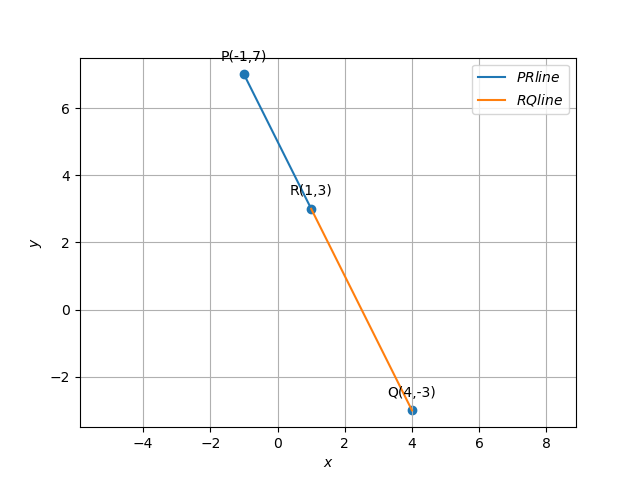
\includegraphics[width=\columnwidth]{chapters/10/7/2/1/figs/linefig.png}
\end{center}
\caption{}
\label{fig:chapters/10/7/2/1/Fig}
\end{figure}

